\chapter{Resultados}

En este capítulo se presentan los resultados obtenidos de la implementación
del sistema. Se comienza presentando los resultados obtenidos por el
extractor de información y presentando la base de datos de \textit{embeddings}
generada. A continuación, se muestra el conjunto de datos de preguntas
y respuestas generado, así como los resultados de las
evaluaciones de los diferentes modelos de extracción de \textit{embeddings}
y de inferencia de respuestas. Posteriormente, se presentan
los resultados del reentrenamiento de los modelos de \textit{embeddings},
para finalmente describir el proceso de puesta en producción del sistema.
En cada paso se discutirán los resultados mostrados, así como los retos y
criterios considerados en la toma de decisiones que llevaron a la
configuración final del sistema en producción.

\section{Extractor de información}

En la metodología se mencionan dos formas de extraer la información de los
documentos normativos, usando \textit{PyPdf+PyTesseract} y empleando
\textit{Pdfplumber}. Ambos métodos tienen como finalidad generar una base
de datos de \textit{embeddings} que contenga toda la información de los
documentos normativos, incluyendo la estrutura de los documentos con
sus títulos y secciones. En las siguientes subsecciones se presentan algunas
de las consideraciones adicionales que se tuvieron que implementar para hacer
la correcta extracción de la información.

\subsection{Eliminación de encabezados y pies de página}

Todos los documentos normativos de la universidad tienen un encabezado con
el nombre del documento y un pie de página con el número de página, esta es
información irrelevante que se desea eliminar. Para eliminar estos elementos
se normaliza a 1.0 el ancho y alto de la página, para posteriormente
establecer los márgenes superior, inferior, izquierdo y derecho como decimales.
Todo el texto que se encuentre fuera de dichos márgenes es ignorado como
se muestra en la figura \ref{fig:quitar_encabezados}. El ancho y alto totales
del documento se obtienen directamente de \textit{PyPdf}, \textit{PyTesseract}
y \textit{Pdfplumber} según sea el caso. La mayoría de los documentos normativos
comparten un márgen de: (izquierda: 0.5, arriba: 0.1, derecha: 0.95, abajo: 0.95),
sin embargo, este parámetro es configurable mediante un archivo YAML para
dar flexibilidad al procesar otros documentos.

\begin{figure}
    \centering
    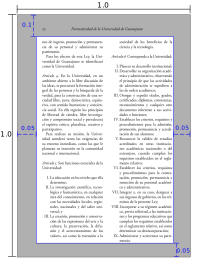
\includegraphics[width = 0.8\textwidth]{\DirFigCcuatro/quitar_encabezados}
    \caption{Elminación de encabezados y pies de página con márgenes.}
    \label{fig:quitar_encabezados}
\end{figure}

\subsection{Detección de títulos centrados}

Durante la implementación de la detección de títulos centrados, la mayoría
de los títulos de los documentos están bien definidos y separados, por lo
que su detección es sencilla como en la figura \ref{fig:titulo_ok}. Sin embargo,
hay ocasiones en las que si se analiza una línea de forma aislada, ésta
parece estar centrada (recuadro rojo de figura \ref{fig:titulo_wrong}), cuando en realidad es parte de una viñeta o un
texto con sangría, es por eso que se opta por hacer el análisis por bloques
separados verticalmente (recuadro verde de figura \ref{fig:titulo_wrong}).
Se determina que un bloque está separado verticalmente cuando hay una distancia
mayor a un valor configurable, proporcional al alto de la línea.

\begin{figure}
    \centering
    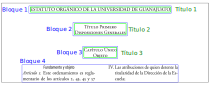
\includegraphics[width = 0.8\textwidth]{\DirFigCcuatro/title_ok}
    \caption{Detección correcta de títulos centrados y agrupación en bloques de texto
        por separación vertical.}
    \label{fig:titulo_ok}
\end{figure}

\begin{figure}
    \centering
    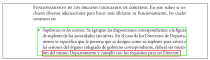
\includegraphics[width = 0.8\textwidth]{\DirFigCcuatro/title_wrong}
    \caption{Línea de texto aparentemente centrada (recuadro rojo) que al
        separar el documento en bloques (recuadro verde) ya no se detecta como título.}
    \label{fig:titulo_wrong}
\end{figure}

El caso de los títulos centrados en la columna es más complejo, pues cuando
el texto es muy extenso, ya no parece estar centrado, como en la figura
\ref{fig:title_column}, por lo que se opta por un enfoque en el que primero
se detecta el bloque de texto, luego se da una tolerancia de $L$ líneas para
detectar el inicio de un artículo con la expresión regular, de ser así,
las $l$ líneas previas son consideradas como un título del artículo.

\begin{figure}
    \centering
    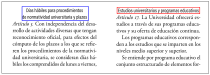
\includegraphics[width = 0.8\textwidth]{\DirFigCcuatro/title_column}
    \caption{Título centrado en columna ideal (izquierda) y título centrado en
        columna que no puede ser detectado como texto centrado (derecha).}
    \label{fig:title_column}
\end{figure}

Por otra parte, el documento correspondiente al modelo educativo de la
universidad, rompe con la estructura de los demás documentos, pues no es un
documento con artículos, sino más bien una guía de la estructura educativa
de la institución, esto no impide que sea dividido en secciones y fragmentos,
pero presenta la diferencia de que es un texto justificado a una columna y
sus secciones son numéricas y no están centradas, por lo que para detectarlas
el texto solamnte se divide en bloques verticales y cada bloque se valida
con una expresión regular como se muestra en la figura \ref{fig:titulo_no_centrado}.
Este comportamiento no interfiere con la detección de títulos centrados
pues ambos procesos se realizan para todos los documentos.

\begin{figure}
    \centering
    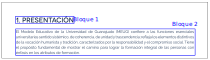
\includegraphics[width = 0.8\textwidth]{\DirFigCcuatro/titulo_no_centrado}
    \caption{Documento con títulos a la izquierda son detectados al separalos
        en bloques verticales y validar contra una expresión regular.}
    \label{fig:titulo_no_centrado}
\end{figure}

En cuanto a la generación del árbol, se realizó adecuadamente para todos los
documentos normativos, sin embargo, el preámbulo de los documentos, al
tener un formato menos regular puede presentar algunas estructuras poco
congruentes, como se observa en el recuadro rojo de la figura
\ref{fig:arbol}, aún así, estas estructuras no afectan el sistema
pues la estructura de capítulos y artículos se genera correctamente,
como se observa en el recuadro verde de la figura \ref{fig:arbol} y
el preámbulo puede ignorarse si así se deseara. Además, en la figura
\ref{fig:arbol_2} se muestra parte de la estructura generada para el documento
``Modelo Educativo de la Universidad de guanajuato y su Modelo Académico''
que, a pesar de que el documento tiene una estructura diferente, puede
procesarse adecuadamente.

\begin{figure}
    \centering
    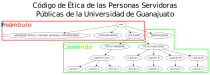
\includegraphics[width = 0.8\textwidth]{\DirFigCcuatro/arbol}
    \caption{Árbol de documento generado automáticamente. Se observa el preámbulo
        con algunos títulos erroneos (recuadro rojo) y el contenido del documento
        detectado correctamente (recuadro verde).}
    \label{fig:arbol}
\end{figure}

\begin{figure}
    \centering
    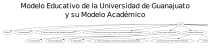
\includegraphics[width = 0.8\textwidth]{\DirFigCcuatro/arbol_2}
    \caption{Árbol de documento ``Modelo Educativo de la Universidad de guanajuato y su Modelo Académico''
        que es un documento a una columna, justificado y con secciones numéricas.}
    \label{fig:arbol_2}
\end{figure}

Por último, para la separación de cada nodo en fragmentos se hicieron
múltiples pruebas para seleccionar el número máximo de caracteres por fragmento.
Estas pruebas consideraron la VRAM disponible, la longitud media y máxima del
contenido de los nodos, entre otros factores. Al final, se encontró que se pueden
usar adecuadamente los modelos de \textit{embeddings} con 2,048 tokens de contexto, lo que
equivale a aproximadamente 8,200 caracteres si se usa el tokenizador de Qwen.
Por lo anterior, el límite de caracteres por fragmento se estableció en 8,000,
ya que al dividirse por párrafos el fragmento más grande resultó de 1,964 tokens.

\section{Conjunto de datos generado}

El conjunto de datos que se generó recopila preguntas y respuestas de
21 documentos diferentes, con un total de 1,082 preguntas y respuestas,
la distribución de preguntas por cada documento se muestra en la figura
\ref{fig:dataset_questions}. Un ejemplo de un registro del conjunto de
datos generado se ve como el siguiente:

\begin{itemize}
    \item \textbf{id:} 81e729afa369916be4d4db99f9c1817c
    \item \textbf{title:} ley-organica-de-la-universidad-de-guanajuato
    \item \textbf{context:} Artículo 1
    \item \textbf{context\_text:} La presente Ley es de orden público y de interés social. Contiene las normas fundamentales de la misión, organización, funcionamiento y gobierno de la Universidad de Guanajuato.
    \item \textbf{question:} ¿Qué contiene la Ley Orgánica de la Universidad de Guanajuato?
    \item \textbf{answers:} \{'text': ['Contiene las normas fundamentales de la misión, organización, funcionamiento y gobierno de la Universidad de Guanajuato']\}
\end{itemize}

\begin{figure}[]
    \centering
    \includegraphics[width = 0.8\textwidth]{\DirFigCcuatro/dataset_questions}
    \caption{Distribución de preguntas por documento.}
    \label{fig:dataset_questions}
\end{figure}

Durante la generación del conjunto de datos se observaron varias particularidades
de los documentos que se tomaron en cuenta para generar las preguntas y se
deberán tener en consideración durante la evaluación de los modelos. Primero,
no fue posible generar preguntas concretas del preámbulo de los documentos,
por lo que estas partes fueron omitidas. Otro elemento particular es la
presencia de artículos transitorios, los cuales, como su nombre lo indica,
son de caracter temporal solo tienen relevancia cuando recién se publica el
documento o la reforma al documento, por lo que incluirlos podría ser
inecesario o contradictorio, pues muchos hacen referencia
a fechas o tiempos de los cuales el sistema no tiene conocimiento. A pesar
de esto, todas las pruebas se realizaron incluyendo estos artículos.

Adicionalmente, en el conjunto de datos se observa cierta tendencia a
que las preguntas contengan las palabras clave al cual están redactadas
en los artículos, usando el nombre completo y apropiado para cada elemento,
ej: ¿Cuáles son las responsabilidades de la persona titular de la Rectoría
General?, cuando sería más natural preguntar ¿Cuáles son las responsabilidades
del Rector General?. Esto podría generar pregunta más fáciles de responder y
con lenguaje un poco alejado del lenguaje común del usuario final.

Finalmente, el conjunto de datos se dividió en dos subconjuntos: entrenamiento
(80\%) y prueba (20\%). El objetivo de esta división es emplear el conjunto de prueba
durante la evaluación de los modelos de \textit{embeddings} reentrenados,
sin embargo, para las demás evaluaciones se empleó el conjunto de datos
completo para evaluar. El conjunto de datos se colocó en un repositorio de
HuggingFace con el objetivo de facilitar su uso en los diferentes equipos
de trabajo, así como su publicación. Usar esta estrategia demostró ser
efectiva pues se pueden conservar diferentes versiones del conjunto de
datos de forma organizada, así como los subconjuntos de entrenamiento y prueba.

\section{Evaluación y selección del modelo de \textit{embeddings}}

Se evaluaron tres modelos diferentes: MiniLM, MPNET y Qwen 3. Del modelo
Qwen 3 se evaluaron sus tres variantes de tamaño: 0.6B, 4B y 8B. Para
cada variante se evaluaron además su versión cuantizada disponible más pequeña y
la más grande, dando como resultados los mostrados en las tabla
\ref{tab:metrics_embedding_top_3} y \ref{tab:metrics_embedding_top_5} para
top-3 y top-5 documentos respectivamente. Se debe considerar que la precision
y la puntuación f1 son naturalmente bajos puesto que cada pregunta del conjunto
de datos fue formulada para que tenga un solo artículo relevante, es decir,
el máximo de fragmentos relevantes por pregunta es 1 o 2 (dado que unos pocos
artículos son de más de un fragmento), de ahí que la mejor
métrica para comparar los modelos sea únicamente el recall.

Si se compara el recall (figuras
\ref{fig:metrics_embedding_top_3}, \ref{fig:metrics_embedding_top_5}), se
puede observar que el mejor modelo es el Qwen3-Embedding-8B, seguido de sus
versiones cuantizadas. Este resultado nos permite seleccionar al modelo
Qwen-Embedding-8B para las siguientes pruebas, así como a su modelo
cuantizado Q4\_K\_M de 4 bits, que con mucha menos memoria alcanza un
rendimiento similar. Por otra parte, se observa la considerable diferencia
de 0.63 y 0.5 puntos de recall entre el mejor modelo y los modelos
all-MiniLM-L6-v2 y multi-qa-mpnet-base-dot-v1 respectivamente. Además,
observamos que existe una diferencia de aproximadamente 0.8 puntos entre
las pruebas con 5 documentos respecto a las de 3 documentos, esto es indicativo
de que no siempre el fragmento relevante real está dentro del top 3, por
lo que alimentar el modelo de inferencia con 5 fragmentos de contexto entregará
mejores resultados sacrificando un poco de memoria para el contexto.

\begin{table}[!ht]
    \centering
    \begin{tabular}{|l|l|l|l|}
        \hline
        Modelo de \textit{embeddings} & precision@3    & recall@3       & f1@3           \\ \hline
        Qwen3-Embedding-0.6B          & 0.184          & 0.549          & 0.274          \\ \hline
        Qwen3-Embedding-0.6B-f16      & 0.248          & 0.743          & 0.371          \\ \hline
        Qwen3-Embedding-0.6B-Q8\_0    & 0.247          & 0.738          & 0.369          \\ \hline
        Qwen3-Embedding-4B            & 0.195          & 0.584          & 0.292          \\ \hline
        Qwen3-Embedding-4B-Q4\_K\_M   & 0.283          & 0.843          & 0.422          \\ \hline
        Qwen3-Embedding-4B-f16        & 0.282          & 0.841          & 0.420          \\ \hline
        \textbf{Qwen3-Embedding-8B}   & \textbf{0.304} & \textbf{0.909} & \textbf{0.454} \\ \hline
        Qwen3-Embedding-8B-Q4\_K\_M   & 0.285          & 0.852          & 0.426          \\ \hline
        Qwen3-Embedding-8B-f16        & 0.286          & 0.855          & 0.427          \\ \hline
        all-MiniLM-L6-v2              & 0.091          & 0.273          & 0.136          \\ \hline
        multi-qa-mpnet-base-dot-v1    & 0.133          & 0.400          & 0.200          \\ \hline
    \end{tabular}
    \caption{Resultados de evaluación para modelos de \textit{embeddings} con $k=3$ documentos relevantes.}
    \label{tab:metrics_embedding_top_3}
\end{table}

\begin{table}[!ht]
    \centering
    \begin{tabular}{|l|l|l|l|}
        \hline
        Modelo de \textit{embeddings} & precision@5    & recall@5       & f1@5  \\ \hline
        Qwen3-Embedding-0.6B          & 0.128          & 0.637          & 0.212 \\ \hline
        Qwen3-Embedding-0.6B-Q8\_0    & 0.169          & 0.840          & 0.280 \\ \hline
        Qwen3-Embedding-0.6B-f16      & 0.169          & 0.840          & 0.280 \\ \hline
        Qwen3-Embedding-4B            & 0.137          & 0.681          & 0.227 \\ \hline
        Qwen3-Embedding-4B-Q4\_K\_M   & 0.186          & 0.919          & 0.306 \\ \hline
        Qwen3-Embedding-4B-f16        & 0.185          & 0.917          & 0.305 \\ \hline
        \textbf{Qwen3-Embedding-8B}   & \textbf{0.198} & \textbf{0.986} & 0.329 \\ \hline
        Qwen3-Embedding-8B-Q4\_K\_M   & 0.185          & 0.919          & 0.306 \\ \hline
        Qwen3-Embedding-8B-f16        & 0.187          & 0.928          & 0.309 \\ \hline
        all-MiniLM-L6-v2              & 0.071          & 0.356          & 0.118 \\ \hline
        multi-qa-mpnet-base-dot-v1    & 0.099          & 0.493          & 0.164 \\ \hline
    \end{tabular}
    \caption{Resultados de evaluación para modelos de \textit{embeddings} con $k=5$ documentos relevantes.}
    \label{tab:metrics_embedding_top_5}
\end{table}

\begin{figure}
    \centering
    \includegraphics[width = 0.8\textwidth]{\DirFigCcuatro/metrics_embedding_top_3}
    \caption{Recall para \textit{embeddings} con top 3 documentos relevantes.}
    \label{fig:metrics_embedding_top_3}
\end{figure}

\begin{figure}
    \centering
    \includegraphics[width = 0.8\textwidth]{\DirFigCcuatro/metrics_embedding_top_5}
    \caption{Recall para \textit{embeddings} con top 5 documentos relevantes.}
    \label{fig:metrics_embedding_top_5}
\end{figure}

\section{Selección de modelo de inferencia}

Para la inferencia se evaluaron tres modelos diferentes: Qwen3 en sus versiones
0.6B y 8B, tanto su versión completa como su versión cuantizada de Q4\_K\_M,
el modelo GPT-OSS 20B y el modelo LLama 3.1 8B. Adicionalmente se evaluó
el modelo de Qwen3 8B con la opción de razonamiento activada. Estas evaluaciones
fueron ejecutadas en el centro de supercómputo del CIMAT, con 48BG de memoria
de video disponibles, además, todos los
modelos fueron evaluados con el top 5 fragmentos relevantes, así como
con el mejor modelo de \textit{embeddings}, es decir, el modelo
Qwen3-Embedding-8B como extractor de \textit{embeddings} de la
pregunta y los fragmentos. Los resultados de esta evaluación se muestran en la
tabla \ref{tab:metrics_inferencia} donde se observa que el mejor modelo es
Qwen3-8B en su versión completa, y de forma interesante, el siguiente modelo
es el Qwen3-0.6B. Nótese que la diferencia en rendimiento es casi igual entre
estos dos modelos y la versión cuantizada de Qwen3-8B, aunque esta emplea requiere
más memoria que Qwen3-0.6B, pero menos que Qwen3-8B.

\begin{table}[!ht]
    \centering
    \begin{tabular}{|l|l|l|l|}
        \hline
        Modelo de inferencia    & RougeL         & Punaje BERT    & Similitud coseno \\ \hline
        Qwen3-0.6B              & 0.412          & 0.774          & 0.677            \\ \hline
        \textbf{Qwen3-8B}       & \textbf{0.424} & \textbf{0.772} & \textbf{0.690}   \\ \hline
        Qwen3-8B-Q4\_K\_M-think & 0.213          & 0.676          & 0.610            \\ \hline
        Qwen3-8B-Q4\_K\_M       & 0.410          & 0.766          & 0.686            \\ \hline
        gpt-oss-20b-MXFP4       & 0.322          & 0.707          & 0.668            \\ \hline
        Llama-3.1-8B-Instruct   & 0.351          & 0.750          & 0.645            \\ \hline
    \end{tabular}
    \caption{Resultados de evaluación de modelos de inferencia con Qwen3-Embedding-8B
        y top 5 documentos.}
    \label{tab:metrics_inferencia}
\end{table}

Una vez obtenidos los resultados de la tabla \ref{tab:metrics_inferencia},
se debe considerar la cantidad de memoria disponible en el servidor
\textit{Dell Precission 90 Tower}, que es de 16GB+2GB+2BG, y se determina que el modelo
Qwen3-Embeddings-8B no puede ejecutarse ahí, por lo que para el siguiente
paso de evaluación se escogieron los tres mejores modelos siguientes, que
son los modelos Qwen3-0.6B, Qwen3-8B-Q4\_K\_M y GPT-OSS-20B. La siguiente
prueba fue mejorar el comando de sistema que se le proporciona al modelo
para hacer ajuste por ingeniería de comandos. Los resultados de esta evaluación
se presentan en la tabla \ref{tab:metrics_prompt}, donde también se evaluó
el modelo Qwen3-8B-Q4\_K\_M con su opción de razonamiento para analizar si
reacciona mejor al haber un comando de sistema más complejo.

\begin{table}[!ht]
    \centering
    \begin{tabular}{|l|l|l|l|}
        \hline
        Modelo                     & RougeL         & Puntaje BERT   & Similitud coseno \\ \hline
        Qwen3-0.6B                 & 0.319          & 0.745          & 0.626            \\ \hline
        Qwen3-8B-Q4\_K\_M          & 0.368          & 0.747          & 0.670            \\ \hline
        Qwen3-8B-Q4\_K\_M-think    & 0.241          & 0.691          & 0.622            \\ \hline
        \textbf{gpt-oss-20b-MXFP4} & \textbf{0.420} & \textbf{0.753} & \textbf{0.707}   \\ \hline
    \end{tabular}
    \caption{Resultados de evaluación de mejores modelos de inferencia con
        comando de sistema más complejo.}
    \label{tab:metrics_prompt}
\end{table}

En la tabla \ref{tab:metrics_prompt} se observa que el modelo GPT-OSS-20B
es el que tiene mejor rendimiento, mostrando una mejora contra la evaluación sin
instrucción de sistema. Por su parte, los modelos Qwen3 empeoraron ligeramente su puntaje
al introducir el comando del sistema. Por último, el modelo Qwen3 con la
opción de razonamiento mejoró ligeramente comparado con su evaluación sin
instrucción, pero no significativamente. Todo lo anterior nos inclina a pensar
que el modelo GPT-OSS-20B es el que mejor se adapta a las instrucciones de sistema,
para verificarlo se procedió a hacer una evaluación manual de las respuestas.
Para la evaluación manual una persona debe, leer la pregunta y comparar la respuesta del modelo
contra la respuesta de referencia, para decidir si la respuesta responde correctamente
a la pregunta, según su criterio. Para esta evaluación se verificaron
25 respuestas aleatorias de los modelos, evaluando la misma pregunta para todos
los modelos con el fin de comparar otros factores como su legibilidad o estilo.
En la tabla \ref{tab:metrics_manual} se muestra el porcentaje de respuestas
correctas para cada uno de los cuatro modelos, aquí se observa que el modelo
Qwen3-0.6B es inferior al resto por un margen considerable, mientras que el
resto se desempeña de una forma muy similar.

\begin{table}[!ht]
    \centering
    \begin{tabular}{|l|r|}
        \hline
        Modelo                           & Aciertos       \\ \hline
        Qwen3-0.6B                       & 60 \%          \\ \hline
        \textbf{GPT-OSS}                 & \textbf{88} \% \\ \hline
        Qwen3-8B-Q4\_K\_M                & 84 \%          \\ \hline
        \textbf{Qwen3-8B-Q4\_K\_M-think} & \textbf{88} \% \\ \hline
    \end{tabular}
    \caption{Porcentaje de respuesta correctas por modelo en una muestra de 25 preguntas aleatorias.}
    \label{tab:metrics_manual}
\end{table}

Para entender la discrepancia de rendimiento entre las métricas cuantitativas
y la evaluación cualitativa del modelo Qwen3-0.6B, se analizaron las respuestas
a profundidad y se encontró que el modelo tiende a cometer ligeras imprecisiones
en las respuesatas, como omitir una fracción, agregar texto que no tiene que
ver con la pregunta o escribir texto incoherente, lo que provoca el evaluador
califique la respuesta como errada, además, se observó que comete errores de
escritura de las palabras con acentos o formateo incorrecto de las respuestas.
Por su parte, la discrepancia de rendimiento del modelo Qwen3-8B-Q4\_K\_M-think
se debe a que el modelo genera respuestas muy extensas (además de cadenas de
razonamiento innecesariamente largas), donde el texto adicional abona contexto
a la respuesta incluyendo detalles adicionales, por lo que un evaluador puede
dar por buena la respuesta aunque textualmente no sea similar a la respuesta
de referencia.

Finalmente, se descarta el modelo Qwen3-0.6B por sus imprecisiones y errores,
así como el modelo Qwen3-8B-Q4\_K\_M porque, si bien las respuestas son correctas,
el texto adicional agregado es una distracción innecesaria. Se hicieron pruebas
adicionales, menos rigurosas sobre los modelos restantes y se determinó que
el modelo GPT-OSS reacciona mejor a los comandos de sistema, es mejor
siguiendo instrucciones y en general su formato de salida es más amigable,
es por ello que se seleccionó este modelo como el modelo de inferencia final
para el sistema.

\section{Reentrenamiento de modelo de \textit{embeddings}}

Dos modelos de embeddings se sometieron a un proceso de reentrenamiento:
all-MiniLM-L6-v2 y multi-qa-mpnet-base-dot-v1. Ambos modelos fueron
reentrenados con el subconjunto de datos de entrenamiento, de este
subconjunto se extrajo un 10\% adicional para validación. El reentrenamiento
se llevó a cabo en el centro de supercómputo del CIMAT donde cada modelo
se reentrenó por un total de 100 épocas con un tamaño de batch de 32.
El subconjunto de prueba se empleó para evaluar los modelos antes y después
del entrenamiento, para tener la comparativa de su mejora. La evaluación
inicial se muestra en la tabla \ref{tab:pre_train}, mientras que la
evaluación final se muestra en la tabla \ref{tab:post_train}.



\section{Puesta en producción}

La puesta en producción del sistema consta de tres componentes: un servidor con GPUs
donde se ejecuten los modelos LLM, un servidor en la nube donde se ejecute la
aplicación web y una VPN (Virtual Private Network) para comunicar ambos
componentes. Para el servidor con GPUS, se emplea la \textit{Dell Precission 7920 Tower}
que se encuentra dentro de las instalaciones de la División de Ingenierías
del Campus Irapuato-Salamanca (DICIS) de la Universidad de Guanajuato, en este servidor
se coloca el extractor de información, el modelador del lenguaje y la API
de comunicación. El servidor en la nube corresponde a una máquina virtual
de Azure del tipo \textit{Standard B2pts v2 (2vcpus, GiB memory)}, con
Ubuntu 24.04, donde se ejecuta la aplicación web. Este servidor debe
ser visible desde internet, por lo se le asigna una IP pública.
Por último, la VPN se configura en Azure para conectar directamente con
la máquina virtual, mientras que \textit{Dell} se conecta a través de
una puerta de enlace VPN. El esquema completo de conexiones se encuentra
en la figura \ref{fig:conexion_prod}.

\begin{figure}
    \centering
    \includegraphics[width = 0.8\textwidth]{\DirFigCcuatro/conexion_prod}
    \caption{Diagrama de conexión de sistema.}
    \label{fig:conexion_prod}
\end{figure}

\subsection{Servidor GPUs}

Este servidor contiene la API de comunicación, el modelador de lenguaje y
el extractor de información. El servidor se configuró con Docker para
hacer el despliegue de los contenedores necesarios. Se creó una imagen de
contenedor llamada \textit{normativity\_rag}, la cual contiene el extractor
de información. Este contenedor tiene la capacidad de ejecutar todos los
scripts relacionados con la extracción de información, ingluido un script
que toma todos los documentos PDF de un directorio y realiza el proceso de
extracción para generar la base de datos en ChromaDB con los \textit{embeddings}.
Hacerlo de esta forma permite usar llama\_cpp en windows, además proporciona
las ventajas propias de los contenedores Docker, como son la posibilidad
de ejecutar la misma imagen en equipos diferentes sin instalar dependencias.
El único requisito que debe cumplir el servidor para funcionar correctamente
es tener instalados los Drivers de Nvidia, en cualquiera de sus versiones, y
tener CUDA 12.3 instalado, es importante que la versión sea la misma pues
debe ser compatible con la imagen del contenedor.

**Dockerfile de normativity\_rag**

En cuanto al modelador del lenguaje y la API de comunicación, ambos se
incluyen en otro contenedor llamado \textit{llm\_api}. A este contenedor
se le mapea el puerto 8080 del servidor para poder acceder a la API desde
la VPN. Para una administración más sencilla del contenedor se crea un archivo
docker-compose.yml en el que se indica el contenedor a usar, el puerto a
mapear y el volumen a cargar donde se encuentra la base de datos de la API
y los modelos descargados. Este contenedor requiere la inicialización de la
base de datos, así como la creación de al menos una API-KEY para acceder,
para ello se ejecuta un script en python dentro del contenedor.

**Dockerfile de llm\_api**

**docker-compose.yml**

La administración de la conexión a la VPN se hace a través de la aplicación
``Azure VPN'', la cual emplea una llave privada, que hay que configurar en el
sistema, y un archivo de configuración para conectarse a la puerta de enlace
VPN configurada en Azure. Una desventaja de esta estructua es que la
conexión a la VPN tiene que hacerse manualmente al encender el servidor,
además, cuando existen problemas de conexión de internet, es posible que la
VPN se desconecte y deba reconectarse manualmente. Otro problema es que
Azure no ofrece una forma directa de configurar una IP estática para un
equipo específico, por lo que cada vez que se reconecta la VPN puede asignar
una IP diferente al servidor y se debe actualizar esta configuración en la
aplicación. Otra desventaja de emplear un servidor local es que éste puede
presentar intermitencia de conexión o fallas en el sumministro de luz.

**Captura Azure VPN**

El contenedor \textit{llm\_api} carga de forma automática los modelos de
\textit{embeddings} e inferencia en la tarjeta gráfica cuando se realiza
la primera petición a la API y utiliza los mismos modelos para todas las
peticiones, por lo que es un posible cuello de botella cuando se tienen
multiples usuarios conectados. El modelo seleccionado para el cálculo
de \textit{embeddings} es el Qwen3-Embedding-8B-Q4\_K\_M, mientras que
el modelo de inferencia es el GPT-OSS-20B-MXFP4, ambos modelos ocupan
15.7 GB de VRAM, por lo que caben en la tarjeta RTX A4000 del servidor.

**uso de memoria**

Por último, el servidor ejecuta Windows, por lo que se debe habilitar
la conexión al puerto 8080 con una regla de sistema.

**Regla puerto 8080**

\subsection{Máquina virtual en la nube}

En la máquina virtual de la nube también se instala Docker para ejecutar los
contenedores necesarios. La aplicación web se coloca en un contenedor con
el puerto 3000 expuesto, la base de datos de la aplicación se coloca en otro
contenedor con el puerto 3306 expuesto y un tercer contenedor con Nginx se
crea para fungir como proxy inverso y controlar el acceso a la aplicación,
además es necesario para configurar los certificados SSL.